\begingroup
\linespread{1}\selectfont
\definecolor{chtomtech}{RGB}{231,126,182}
\definecolor{chtomcivic}{RGB}{155,91,163}
\definecolor{chtomfamily}{RGB}{117,189,174}
\definecolor{chtomwork}{RGB}{247,230,166}
\definecolor{chtomschool}{RGB}{139,133,186}
\definecolor{chtomneigh}{RGB}{229,130,115}
\definecolor{chtomrecreation}{RGB}{95,144,190}
\definecolor{chtomfriend}{RGB}{238,152,63}
\definecolor{chtomromance}{RGB}{164,208,81}
\definecolor{chtomink}{RGB}{42,52,78}
\resizebox{0.99\linewidth}{!}{%
\begin{tikzpicture}[x=0.01cm,y=-0.01cm,
  every node/.style={inner sep=0pt,outer sep=0pt},
  chout/.style={font=\fontsize{6.3pt}{7.2pt}\selectfont},
  chin/.style={font=\bfseries\fontsize{7pt}{8pt}\selectfont,text=chtomink}]
\begin{scope}
\clip (0,0) rectangle (1180,850);
\node[anchor=north west] at (0,0) {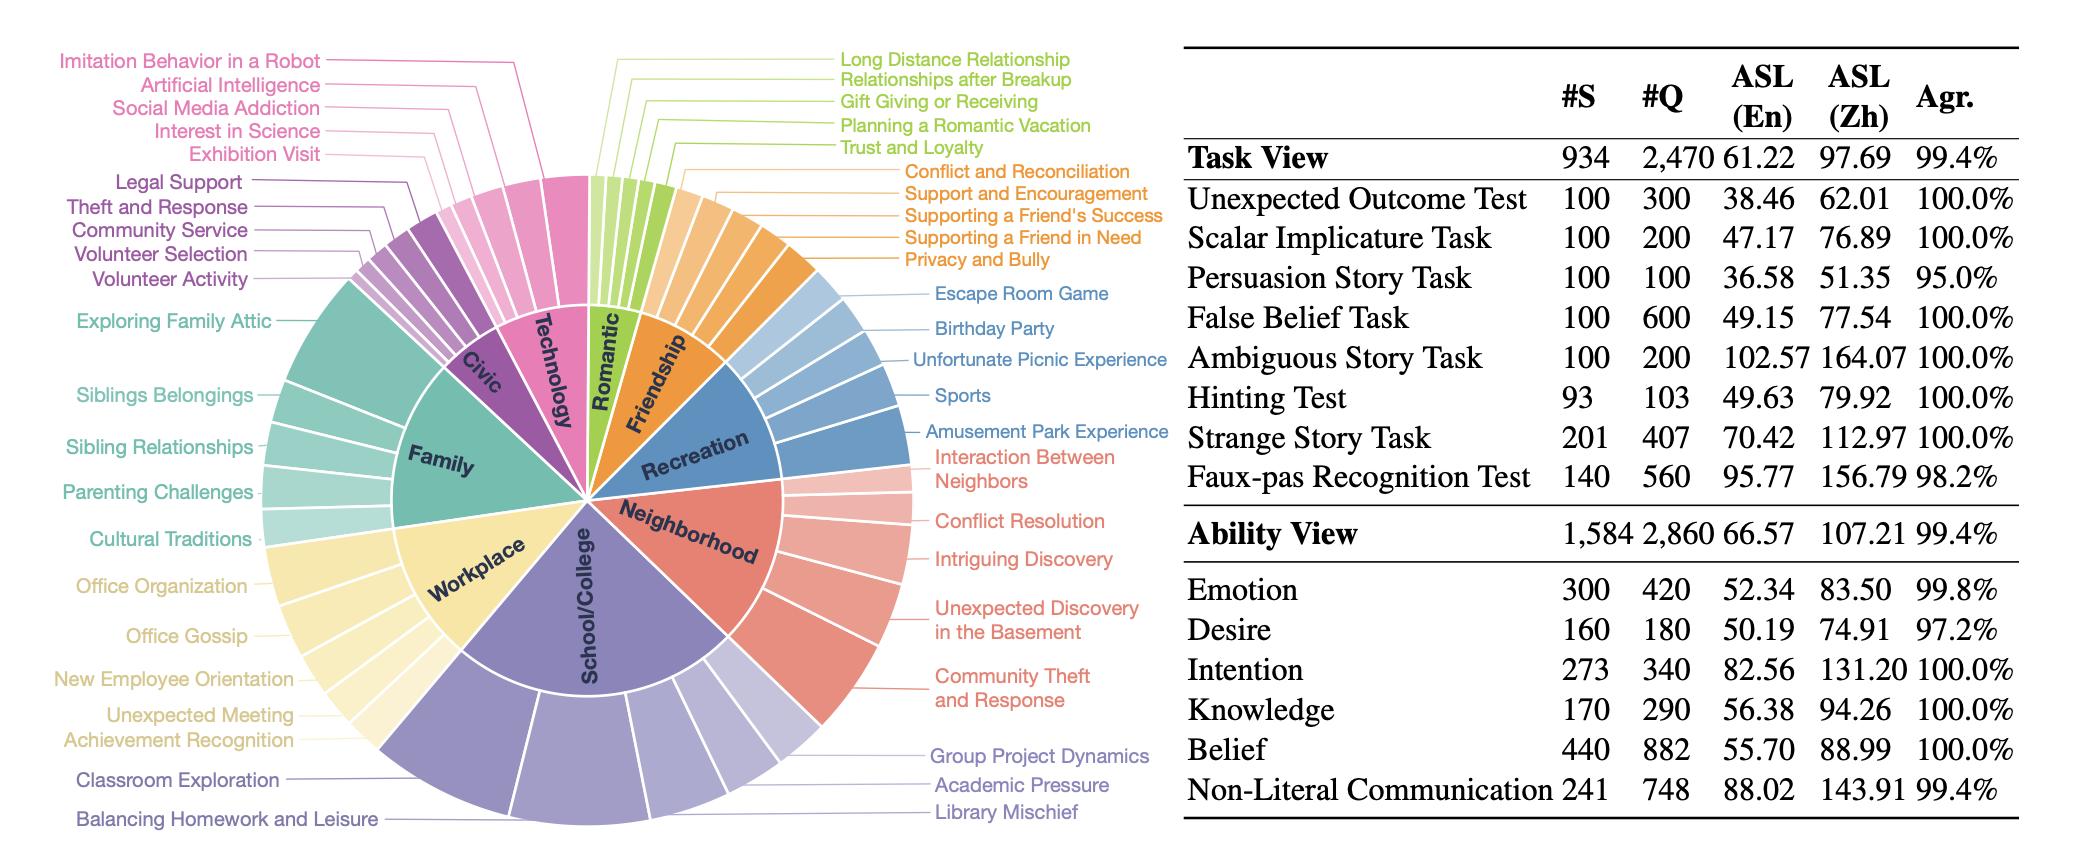
\includegraphics[width=20.78cm]{figures/tombench.png}};
\end{scope}
\fill[white] (15,44) rectangle (325,168);
\node[chout,anchor=east,text=chtomtech] at (321,60) {机器人模仿行为};
\node[chout,anchor=east,text=chtomtech] at (321,84) {人工智能};
\node[chout,anchor=east,text=chtomtech] at (321,107) {社交媒体成瘾};
\node[chout,anchor=east,text=chtomtech] at (321,130) {对科学的兴趣};
\node[chout,anchor=east,text=chtomtech] at (321,154) {参观展览};
\fill[white] (15,170) rectangle (251,287);
\node[chout,anchor=east,text=chtomcivic] at (248,182) {法律支持};
\node[chout,anchor=east,text=chtomcivic] at (248,206) {盗窃及其应对};
\node[chout,anchor=east,text=chtomcivic] at (248,230) {社区服务};
\node[chout,anchor=east,text=chtomcivic] at (248,254) {志愿者选拔};
\node[chout,anchor=east,text=chtomcivic] at (248,278) {志愿活动};
\fill[white] (15,307) rectangle (274,335);
\node[chout,anchor=east,text=chtomfamily] at (271,321) {探索家中阁楼};
\fill[white] (15,379) rectangle (255,407);
\node[chout,anchor=east,text=chtomfamily] at (252,394) {兄弟姐妹的物品};
\fill[white] (15,433) rectangle (259,461);
\node[chout,anchor=east,text=chtomfamily] at (256,448) {手足关系};
\fill[white] (15,477) rectangle (258,506);
\node[chout,anchor=east,text=chtomfamily] at (255,492) {育儿挑战};
\fill[white] (15,524) rectangle (254,553);
\node[chout,anchor=east,text=chtomfamily] at (251,539) {文化传统};
\fill[white] (15,571) rectangle (253,601);
\node[chout,anchor=east,text=chtomwork!80!black] at (250,586) {办公室组织};
\fill[white] (15,622) rectangle (255,650);
\node[chout,anchor=east,text=chtomwork!80!black] at (252,637) {办公室闲谈};
\fill[white] (15,665) rectangle (295,693);
\node[chout,anchor=east,text=chtomwork!80!black] at (292,679) {新员工入职培训};
\fill[white] (15,700) rectangle (297,728);
\node[chout,anchor=east,text=chtomwork!80!black] at (294,715) {意外会面};
\fill[white] (15,729) rectangle (332,756);
\node[chout,anchor=east,text=chtomwork!80!black] at (329,742) {成就认可};
\fill[white] (15,767) rectangle (379,794);
\node[chout,anchor=east,text=chtomschool] at (376,780) {课堂探索};
\fill[white] (15,806) rectangle (509,835);
\node[chout,anchor=east,text=chtomschool] at (506,820) {平衡作业与休闲};
\fill[white] (838,43) rectangle (1178,158);
\node[chout,anchor=west,text=chtomromance!85!black] at (841,58) {异地恋};
\node[chout,anchor=west,text=chtomromance!85!black] at (841,80) {分手后的关系};
\node[chout,anchor=west,text=chtomromance!85!black] at (841,102) {赠送或接受礼物};
\node[chout,anchor=west,text=chtomromance!85!black] at (841,125) {规划浪漫假期};
\node[chout,anchor=west,text=chtomromance!85!black] at (841,147) {信任与忠诚};
\fill[white] (903,158) rectangle (1178,274);
\node[chout,anchor=west,text=chtomfriend!90!black] at (906,171) {冲突与和解};
\node[chout,anchor=west,text=chtomfriend!90!black] at (906,194) {支持与鼓励};
\node[chout,anchor=west,text=chtomfriend!90!black] at (906,216) {支持朋友的成功};
\node[chout,anchor=west,text=chtomfriend!90!black] at (906,239) {支持有困难的朋友};
\node[chout,anchor=west,text=chtomfriend!90!black] at (906,261) {隐私与欺凌};
\fill[white] (912,279) rectangle (1178,835);
\node[chout,anchor=west,text=chtomrecreation] at (934,294) {密室逃脱游戏};
\node[chout,anchor=west,text=chtomrecreation] at (934,330) {生日聚会};
\node[chout,anchor=west,text=chtomrecreation] at (934,360) {不幸的野餐经历};
\node[chout,anchor=west,text=chtomrecreation] at (934,395) {体育运动};
\node[chout,anchor=west,text=chtomrecreation] at (934,431) {游乐园经历};
\node[chout,anchor=west,text=chtomneigh] at (934,463) {邻里交往};
\node[chout,anchor=west,text=chtomneigh] at (934,522) {冲突解决};
\node[chout,anchor=west,text=chtomneigh] at (934,561) {引人好奇的发现};
\node[chout,anchor=west,text=chtomneigh] at (934,620) {地下室中的意外发现};
\node[chout,anchor=west,text=chtomneigh] at (934,688) {社区盗窃及其应对};
\node[chout,anchor=west,text=chtomschool] at (934,756) {小组项目中的互动};
\node[chout,anchor=west,text=chtomschool] at (934,785) {学业压力};
\node[chout,anchor=west,text=chtomschool] at (934,814) {图书馆恶作剧};
\begin{scope}[shift={(588,501)}]
\path[fill=chtomneigh,draw=white,line width=0.65pt]
  (0,0)--(353.35:195.5) arc[start angle=353.35,end angle=404.15,radius=195.5]--cycle;
\path[fill=chtomschool,draw=white,line width=0.65pt]
  (0,0)--(44.15:195.5) arc[start angle=44.15,end angle=130.65,radius=195.5]--cycle;
\path[fill=chtomwork,draw=white,line width=0.65pt]
  (0,0)--(130.65:195.5) arc[start angle=130.65,end angle=172.05,radius=195.5]--cycle;
\path[fill=chtomfamily,draw=white,line width=0.65pt]
  (0,0)--(172.05:195.5) arc[start angle=172.05,end angle=222.8,radius=195.5]--cycle;
\path[fill=chtomcivic,draw=white,line width=0.65pt]
  (0,0)--(222.8:195.5) arc[start angle=222.8,end angle=242.1,radius=195.5]--cycle;
\path[fill=chtomtech,draw=white,line width=0.65pt]
  (0,0)--(242.1:195.5) arc[start angle=242.1,end angle=270.15,radius=195.5]--cycle;
\path[fill=chtomromance,draw=white,line width=0.65pt]
  (0,0)--(270.15:195.5) arc[start angle=270.15,end angle=285.5,radius=195.5]--cycle;
\path[fill=chtomfriend,draw=white,line width=0.65pt]
  (0,0)--(285.5:195.5) arc[start angle=285.5,end angle=314.55,radius=195.5]--cycle;
\path[fill=chtomrecreation,draw=white,line width=0.65pt]
  (0,0)--(314.55:195.5) arc[start angle=314.55,end angle=353.35,radius=195.5]--cycle;
\end{scope}
\node[chin,rotate=-76] at (553,369) {技术};
\node[chin,rotate=-48] at (488,378) {公民生活};
\node[chin,rotate=-15] at (444,458) {家庭};
\node[chin,rotate=31] at (476,570) {职场};
\node[chin,rotate=90] at (586,606) {学校／大学};
\node[chin,rotate=-22] at (686,532) {邻里};
\node[chin,rotate=23] at (697,449) {娱乐};
\node[chin,rotate=63] at (653,380) {友谊};
\node[chin,rotate=82] at (606,366) {恋爱};
\end{tikzpicture}%
}
\par\vspace{4pt}
{\fontsize{8.5pt}{10.2pt}\selectfont
\setlength{\tabcolsep}{5pt}
\renewcommand{\arraystretch}{1.03}
\begin{tabularx}{0.99\linewidth}{@{}Xrrrrr@{}}
\toprule
 & \#S & \#Q & ASL（En） & ASL（Zh） & Agr. \\
\midrule
\textbf{任务视角} & 934 & 2,470 & 61.22 & 97.69 & 99.4\% \\
非预期结果测试 & 100 & 300 & 38.46 & 62.01 & 100.0\% \\
等级含意任务 & 100 & 200 & 47.17 & 76.89 & 100.0\% \\
说服故事任务 & 100 & 100 & 36.58 & 51.35 & 95.0\% \\
错误信念任务 & 100 & 600 & 49.15 & 77.54 & 100.0\% \\
模糊故事任务 & 100 & 200 & 102.57 & 164.07 & 100.0\% \\
暗示测试 & 93 & 103 & 49.63 & 79.92 & 100.0\% \\
奇怪故事任务 & 201 & 407 & 70.42 & 112.97 & 100.0\% \\
失言识别测试 & 140 & 560 & 95.77 & 156.79 & 98.2\% \\
\midrule
\textbf{能力视角} & 1,584 & 2,860 & 66.57 & 107.21 & 99.4\% \\
\midrule
情绪 & 300 & 420 & 52.34 & 83.50 & 99.8\% \\
愿望 & 160 & 180 & 50.19 & 74.91 & 97.2\% \\
意图 & 273 & 340 & 82.56 & 131.20 & 100.0\% \\
知识 & 170 & 290 & 56.38 & 94.26 & 100.0\% \\
信念 & 440 & 882 & 55.70 & 88.99 & 100.0\% \\
非字面沟通 & 241 & 748 & 88.02 & 143.91 & 99.4\% \\
\bottomrule
\end{tabularx}
}
\endgroup
